\documentclass[12pt,a4paper]{book}
\usepackage{graphicx}

\begin{document}
\newcommand{\gLinear}{gLinear}
\newcommand{\ident}[1]{\texttt{#1}}
\title{\gLinear -- Manual}
\author{G. Esterhuizen}
\maketitle

\chapter{Programmer's Guide}

\section{Object Layout}
Class members are divided into 3 different groups.

\begin{description}
  \item [Generic Interfaces and Algorithms]
    This interface consists of a number of public methods that provides
    a minimum interface required of all descendant classes. This
    includes functions like \ident{size}, \ident{resize}, \ident{alias}
    and \ident{deepen} of the \ident{gVectorBase} class. The
    implementation of the functions is delegated to the base class
    \emph{Required Specialized Implementation} functions through the
    static polymorphism mechanism (Section \ref{sec:static.poly}). This
    allows general policies to be implemented in the top-level class
    without undue code replication. An example of a high-level policy is
    seen in the \ident{resize()} function present in
    \ident{gVectorBase}. This function performs a number of checks
    before calling the specialized resize function
    \ident{specialResize()} of the derived class. Generic Algorithms are
    implemented in terms of the interface functions, making it easy to
    write an efficient algorithm that can be used irrespective of the
    low-level implemetation details. An example of such an algorithm is
    the \ident{min}, \ident{max} and \ident{findElem} functions of the
    \ident{gVectorBase} class. Each algorithm is implemented in exactly
    the same way for all types of vectors, with the only difference
    being the type of the iterator used to access the elements and the
    operator used to compare the elements. These types are deduced from
    the template parameters (which is known at compile-time), allowing a
    generic implementation for the algorithm.
    
  \item [Required Specialized Implementations]
    These functions make up the core of each specialized class. Each
    function contains a minimal implementation that does a very specific
    task. Index checking and other higher-level functions are not performed
    here. The functions are not meant to be called directly from the
    application level, but rather as support functions from a Generic
    Algorithm. The names of the functions are similar to the public generic
    interface that it supports, with the difference that all the functions
    in this group starts with the word \ident{special} e.g.
    \ident{specialAlias} and \ident{specialSize}.
    
  \item [Specialized Interfaces and Data]
    Specialized interfaces are all those interfaces and data members that
    are supported by a certain specialization but not nesessary by the
    others. It also contains the constructors, destructors and assigment
    operator function as these are not inherited.
    
  \item [Constructors and Support]
    
\end{description}

\begin{figure}[htb]
    \fbox{\includegraphics[width=10cm]{classes.eps}}
    \caption{\small{Macro structure of classes}}
    \label{fig:classes.macro}
\end{figure}

\subsection{Constructors and Support}
The following constuctors and support functions are provided by most classes:

\begin{description}
  \item [Default Constuctor] 
    Initializes all values to zero.
  \item [No Init Constructor] 
    Skips all stages of the initialization process. Typically assigns all
    pointers NULL and all  integral and floating-point values zero. This
    constuctor is invoked by passing a single parameter of type
    \emph{gLinearNoInit} to the constructor. Invokes the base class
    \emph{No Init Constructor}.
  \item [Copy Constructor]
    Constructs a new object to be a shallow copy of the argument. Invokes
    the base class \emph{Copy Constructor}.
  \item [Initializing Constructor]
    Constructs and initalizes with the supplied parameters. This is intended for
    internal use and should be protected. This is normally called with a
    list of values, one for each data member of this class and some for
    the base class data. Base class initialization is delegated to the
    base class \emph{Initializing Constructor}.
  \item [Configure Function]
    Used in the same fashion as the \emph{Initializing Constructor} and
    has the same function signature. After calling this, the state of the
    object is the same as it would have been if it had been constructed
    with the same argument list. It is used for off-line configuration or
    construction. It directly implements and requires the
    \emph{Initializing Constructor} as it uses explicit destruction
    followed by placement new to perform the initalization. It calls the
    base class \emph{Configure} function to perform base-class
    inititialization.
  \item [Assignment Operator]
    The assignent operator is listed here because it also doesn't inherit
    and has to be declared in each derived class. To facilitate code
    reuse, a generic implementation of an assignment operator is defined in the
    base class, and the derived class simply forwards the call up to base (which
    was exactly what happens in the case of a normal function declared in the
    base and not overrided in the derived class).
\end{description}

\section{Naming Convention for Identifiers}
A simple naming convention is implemented for the names of all identifiers.

\subsection{Classes}
A class name consists of words delimited by capital letters. \\
Example:
\begin{center} 
    class \textbf{RefCntStorage}$<$T$>$ 
\end{center}
It is desirable to have all class names start in capital letters. An
exception is made in the case of all class names starting in a small {\emph
  g}, e.g. gVector, gMatrix. \\
Example:
\begin{center} 
    class \textbf{gVectorBase}$<$T$>$ 
\end{center}

\subsection{Generic Types}
Generic types, e.g. iterator types, are normally declared as typedefs inside classes.
Identifiers start with a {\emph T\_} prefix, followed by one or more words
delimited by capital letters.
Example:
\begin{center} 
    \textbf{T\_Iterator} begin(void) 
\end{center}

\subsection{Member Functions (Methods) and Data}
Class member functions (methods) and class data members are represented by identifiers delimited by
capital letters. The first letter is \emph{never} capitalized. \\
Example:
\begin{center} 
    T\_Index \textbf{stride} 
\end{center}
\begin{center} 
    T\_Index \textbf{getStride}(void) 
\end{center}

\subsection{Formal Parameters}
Formal parameters follow the same guidelines as data members.

\section{Static Polymorphism}
\label{sec:static.poly}

\section{Constness}

\end{document}  
